\documentclass[12pt]{article}

\usepackage[margin=1in]{geometry}
\usepackage{amsmath,amsthm,amssymb}
\usepackage{mathrsfs}
\usepackage{enumitem}
\usepackage{physics}

\usepackage{tikz}
\usetikzlibrary{calc,decorations.markings}

\newcommand{\magsq}[1]{\big|#1\big|^2}
\newcommand{\avg}[1]{\left<#1\right>}
\newcommand{\fullint}{\int_{-\infty}^\infty}
\newcommand{\fullintd}[1]{\fullint\dd#1\:}
\newcommand{\cint}[2]{\int_{#1}^{#2}}
\newcommand{\cintd}[3]{\cint{#1}{#2}\dd#3\:}

\newcommand{\tens}[1]{\overset{\leftrightarrow}{#1}}

\def\Xint#1{\mathchoice
   {\XXint\displaystyle\textstyle{#1}}%
   {\XXint\textstyle\scriptstyle{#1}}%
   {\XXint\scriptstyle\scriptscriptstyle{#1}}%
   {\XXint\scriptscriptstyle\scriptscriptstyle{#1}}%
   \!\int}
\def\XXint#1#2#3{{\setbox0=\hbox{$#1{#2#3}{\int}$}
     \vcenter{\hbox{$#2#3$}}\kern-.5\wd0}}
\def\ddashint{\Xint=}
\def\dashint{\Xint-}

\newcommand{\fulldashintd}[1]{\dashint_{-\infty}^{\infty}\dd{#1}}

\begin{document}
	
\title{Homework 4}
\author{Sean Ericson \\ Phys 633}
\maketitle

\section*{Problem 1}
\begin{align*}
    \fullintd{x}\frac{f(x)}{x+i0^+} - \mathscr{P} \fullintd{x}\frac{1}{x} &= \fullintd{x}\frac{1}{x+i0^+} - \frac{1/2}{1+i0^+} - \frac{1/2}{x-i0^+} \\
    &= \frac{1}{2}\fullintd{x}\left[\frac{1}{x+i0^+} - \frac{1}{x-i0^+}\right] \\
    &= \frac{1}{2}(-2\pi i f(0)) \\
    &= -\pi i f(0)
\end{align*}
Where the following contour was used:
\begin{center}
    \resizebox{250pt}{!}{
        \begin{tikzpicture}
            \draw (0,-2.5) -- (0,2.5);  % Axis
            \draw (-5.5,0) -- (5.5,0);   
            \foreach \y in {-5,...,5} {
            \draw (\y,-4pt) -- (\y,4pt) node[pos=0,below] {\y};
            }
            \foreach \y in {-2,-1,1,2}{
                \draw (-4pt,\y) -- (4pt,\y) node[pos=0,left] {\y $i$};
            }
            
            \node at (0,0) {$\times$}; % Pole
            
            \draw[thick,red,
            decoration={ markings,  % This schema allows for fine-tuning the positions of arrows
            mark=at position 0.5 with {\arrow{latex}}}, 
            postaction={decorate}]
            (-5,0.75) -- (5,0.75);

            \draw[thick,red,
            decoration={ markings,  % This schema allows for fine-tuning the positions of arrows
            mark=at position 0.5 with {\arrow{latex}}}, 
            postaction={decorate}]
            (-5,-0.75) -- (-5,0.75);
        
            \draw[thick,red,
            decoration={ markings,  % This schema allows for fine-tuning the positions of arrows
            mark=at position 0.5 with {\arrow{latex}}}, 
            postaction={decorate}]
            (5,-0.75) -- (-5,-0.75);

            \draw[thick,red,
            decoration={ markings,  % This schema allows for fine-tuning the positions of arrows
            mark=at position 0.5 with {\arrow{latex}}}, 
            postaction={decorate}]
            (5,0.75) -- (5,-0.75);

        \end{tikzpicture}
    }
\end{center}


\begin{align*}
    \fullintd{x}\frac{f(x)}{x-i0^+} - \mathscr{P} \fullintd{x}\frac{1}{x} &= \fullintd{x}\frac{1}{x-i0^+} - \frac{1/2}{1+i0^+} - \frac{1/2}{x-i0^+} \\
    &= \frac{1}{2}\fullintd{x}\left[\frac{1}{x-i0^+} - \frac{1}{x+i0^+}\right] \\
    &= \frac{1}{2}(2\pi i f(0)) \\
    &= \pi i f(0)
\end{align*}
Where the following contour integral was used:
\begin{center}
    \resizebox{250pt}{!}{
        \begin{tikzpicture}
            \draw (0,-2.5) -- (0,2.5);  % Axis
            \draw (-5.5,0) -- (5.5,0);   
            \foreach \y in {-5,...,5} {
            \draw (\y,-4pt) -- (\y,4pt) node[pos=0,below] {\y};
            }
            \foreach \y in {-2,-1,1,2}{
                \draw (-4pt,\y) -- (4pt,\y) node[pos=0,left] {\y $i$};
            }
            
            \node at (0,0) {$\times$}; % Pole
            
            \draw[thick,red,
            decoration={ markings,  % This schema allows for fine-tuning the positions of arrows
            mark=at position 0.5 with {\arrow{latex}}}, 
            postaction={decorate}]
            (5,0.75) -- (-5,0.75);

            \draw[thick,red,
            decoration={ markings,  % This schema allows for fine-tuning the positions of arrows
            mark=at position 0.5 with {\arrow{latex}}}, 
            postaction={decorate}]
            (-5,0.75) -- (-5,-0.75);
        
            \draw[thick,red,
            decoration={ markings,  % This schema allows for fine-tuning the positions of arrows
            mark=at position 0.5 with {\arrow{latex}}}, 
            postaction={decorate}]
            (-5,-0.75) -- (5,-0.75);

            \draw[thick,red,
            decoration={ markings,  % This schema allows for fine-tuning the positions of arrows
            mark=at position 0.5 with {\arrow{latex}}}, 
            postaction={decorate}]
            (5,-0.75) -- (5,0.75);

        \end{tikzpicture}
    }
\end{center}
Thus
\[ \fullintd{x} \frac{f(x)}{x\pm i0^+} - \mathscr{P}\fullintd{x}\frac{f(x)}{x} = \mp i\pi f(0) \]
\[ \implies \]
\[ \frac{1}{x\pm i0^+} = \mathscr{P}\frac{1}{x} \mp i\pi\delta(x) \]

\section*{Problem 2}
Given that 
\[ \tens{\chi}(\omega) - \tens{\chi}_0 = \frac{1}{\pi i} \dashint_{-\infty}^{\infty}\dd{\omega'} \frac{\tens{\chi}(\omega')-\tens{\chi}_0}{\omega' - \omega} \]
we have
\begin{align*}
    \frac{1}{\pi}\fulldashintd{\omega'} \frac{\tens{\zeta}(\omega') - \tens{\chi}_0}{\omega' - \omega} &= \frac{1}{\pi}\fulldashintd{\omega'}\frac{\tens{\chi}(\omega') - \tens{\chi}_0}{\omega' - \omega} + \frac{i}{\pi}\fulldashintd{\omega'}\frac{\tens{\sigma}(\omega')}{\omega'(\omega' - \omega)} \\
    &= i(\tens{\chi}(\omega) - \tens{\chi}_0) - \frac{\tens{\sigma}(\omega)}{\omega} + \frac{\tens{\sigma}_0}{\omega} \\
    &= i\left(\tens{\zeta}(\omega) - \tens{\chi}_0 - \frac{i\tens{\sigma}_0}{\omega}\right)
\end{align*}
Therefore
\[ \tens{\zeta}(\omega) - \tens{\chi}_0 = \frac{1}{\pi i}\fulldashintd{\omega'}\frac{\tens{\zeta}(\omega') - \tens{\chi}_0}{\omega' - \omega} + \frac{i\tens{\sigma}_0}{\omega} \]
while splitting up the real and imaginary parts gives
\begin{alignat*}{2}
    \Re[\tens{\zeta}(\omega) - \tens{\chi}_0] &= &&\frac{1}{\pi}\fulldashintd{\omega'}\frac{\Im[\tens{\zeta}(\omega) - \tens{\chi}_0]}{\omega' - \omega} \\
    \Im[\tens{\zeta}(\omega) - \tens{\chi}_0] &= -&&\frac{1}{\pi}\fulldashintd{\omega'}\frac{\Re[\tens{\zeta}(\omega) - \tens{\chi}_0]}{\omega' - \omega}  + \frac{\tens{\sigma}_0}{\omega}
\end{alignat*}

\section*{Problem 3}
Firstly,
\[ \tens{\chi}(-\omega^*) = \frac{i}{\hbar}\cintd{0}{\infty}{\tau}\ev{\comm{\tilde{x}_\alpha(\tau)}{\tilde{x}_\beta(0)}}e^{-i\omega^*\tau} \]
\[ \tens{\chi}^*(\omega) = -\frac{i}{\hbar}\cintd{0}{\infty}{\tau}\ev{\comm{\tilde{x}_\beta(0)}{\tilde{x}_\alpha(\tau)}}e^{-i\omega^*\tau} = \frac{i}{\hbar}\cintd{0}{\infty}{\tau}\ev{\comm{\tilde{x}_\alpha(\tau)}{\tilde{x}_\beta(0)}}e^{-i\omega^*\tau} \]
so we have 
\[  \tens{\chi}(-\omega^*) = \tens{\chi}^*(\omega) \]
This means, for a real frequency $\omega$, $\Re[\tens{\chi}(\omega)]$ is an even function, while $\Im[\tens{\chi}(\omega)]$ is odd. Now, noting that $\tens{\chi_0}$ must be real,
\begin{align*}
    \Re[\tens{\chi}(\omega)] &= \tens{\chi}_0 + \frac{1}{\pi}\fulldashintd{\omega'}\frac{\Im[\tens{\chi}(\omega')]}{\omega' - \omega} \\
    &= \tens{\chi}_0 + \frac{1}{\pi}\fulldashintd{\omega'}\frac{\Im[\tens{\chi}(\omega')]}{\omega'^2 - \omega^2}(\omega' + \omega) \\
    &= \tens{\chi}_0 + \frac{1}{\pi}\fulldashintd{\omega'}\frac{\omega'\Im[\tens{\chi}(\omega')]}{\omega'^2 - \omega^2} + \frac{\omega}{\pi}\fulldashintd{\omega'}\frac{\Im[\tens{\chi}(\omega')]}{\omega'^2-\omega^2} \\
    &= \tens{\chi}_0 + \frac{2}{\pi}\dashint_0^\infty\dd{\omega'}\frac{\omega'\Im[\tens{\chi}(\omega')]}{\omega'^2 - \omega^2}
\end{align*}
Where, in the second to last line, the second integral vanishes due to $\Im[\tens{\chi}(\omega')]$ being odd, while the evenness of $\Re[\tens{\chi}(\omega')]$ allows the domain of the first integral to be restricted to the positive reals (with an additional factor of 2). \\
Similarly,
\begin{align*}
    \Im[\tens{\chi}(\omega)] &= -\frac{1}{\pi}\fulldashintd{\omega'}\frac{\Re[\tens{\chi}(\omega')] - \tens{\chi}_0}{\omega' - \omega} \\
    &= -\frac{1}{\pi}\fulldashintd{\omega'}\frac{\Re[\tens{\chi}(\omega')] - \tens{\chi}_0}{\omega'^2 - \omega^2}(\omega' + \omega) \\
    &= -\frac{1}{\pi}\fulldashintd{\omega'}\frac{\omega'\left(\Re[\tens{\chi}(\omega')] + \tens{\chi}_0\right)}{\omega'^2 - \omega^2} - \frac{\omega}{\pi}\fulldashintd{\omega'}\frac{\Re[\tens{\chi}(\omega')] - \tens{\chi}_0}{\omega'^2 - \omega^2} \\
    &= -\frac{2\omega}{\pi}\dashint_0^\infty\dd{\omega'}\frac{\Re[\tens{\chi}(\omega')] - \tens{\chi}_0}{\omega'^2 - \omega^2} 
\end{align*}

\section*{Problem 4}
\begin{enumerate}[label=(\alph*)]
    \item
    By the definition of the Green's function,
    \[ \left(\pdv[2]{t} + \gamma\pdv{t} + \omega_0^2\right)g(t,t') = \delta(t-t'). \]
    Taking the Fourier transform of the above equation (with respect to $t$) yields
    \[ \left(-\omega^2 - i\gamma\omega + \omega_0^2\right)g(\omega,t') = \fullintd{t}\delta(t-t')e^{i\omega t} = e^{i\omega t'} \]
    \[ \implies  \]
    \begin{equation}
        \label{eq1}
        g(\omega, t') = \frac{e^{i\omega t'}}{-\omega^2 - i\gamma\omega + \omega_0^2}
    \end{equation} 
    Inverting the Fourier transform gives
    \begin{align*}
        g(t, t') &= -\frac{1}{2\pi}\fullintd{\omega}\frac{e^{i\omega t'}e^{-i\omega t}}{\omega^2 + i\gamma\omega - \omega_0^2} \\
        &= -\frac{1}{2\pi}\fullintd{\omega}\frac{e^{-i\omega(t-t')}}{(\omega-\omega_+)(\omega - \omega_-)}
    \end{align*}
    where
    \[ \omega_\pm = -\frac{i\gamma}{2} \pm \tilde{\omega}; \quad \tilde{\omega} = \sqrt{\omega_0^2 - \frac{\gamma^2}{4}} \]
    This integral can be calculated using Cauchy's residue theorem by considering the contours below:
    \begin{center}
        \resizebox{250pt}{!}{
            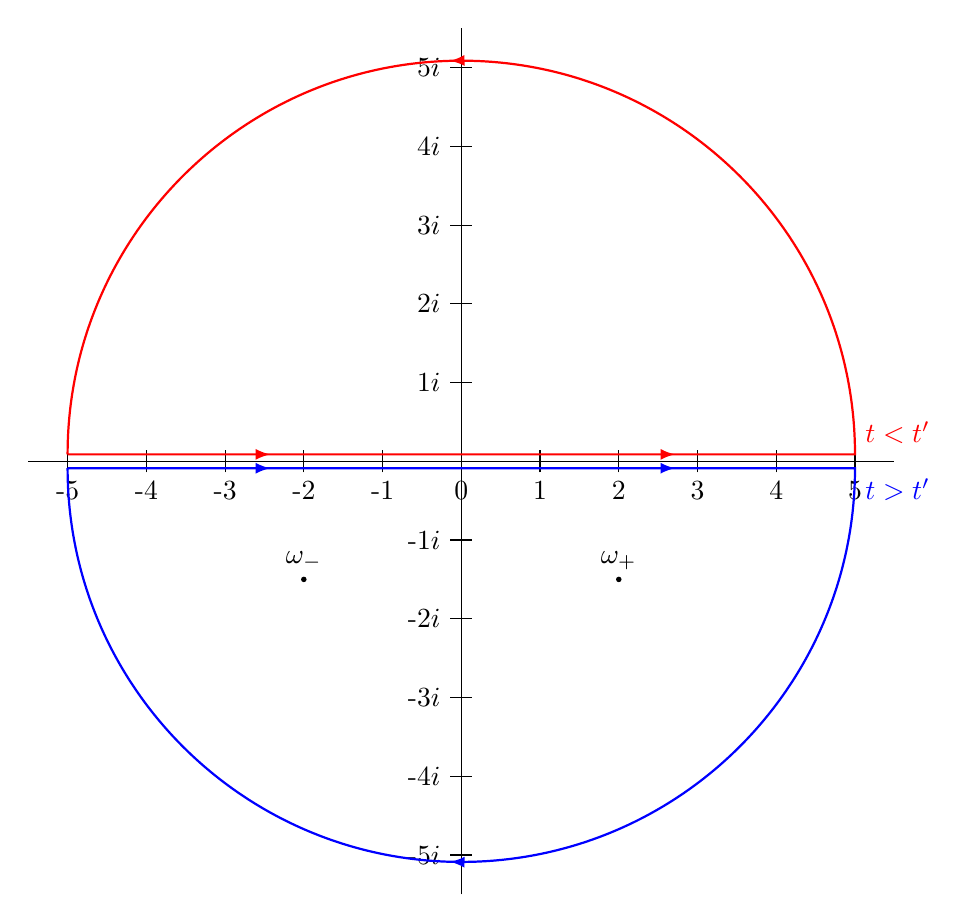
\begin{tikzpicture}
                \draw (0,-5.5) -- (0,5.5);  % Axis
                \draw (-5.5,0) -- (5.5,0);   
                \foreach \y in {-5,...,5} {
                \draw (\y,-4pt) -- (\y,4pt) node[pos=0,below] {\y};
                }
                \foreach \y in {-5,-4,-3,-2,-1,1,2,3,4,5}{
                    \draw (-4pt,\y) -- (4pt,\y) node[pos=0,left] {\y $i$};
                }
                
                \node[fill,circle,inner sep=0pt, minimum width=2pt] (A) at (-2,-1.5) {};
                \node[above] at (A) {$\omega_-$};
                \node[fill,circle,inner sep=0pt, minimum width=2pt] (A) at (2,-1.5) {};
                \node[above] at (A) {$\omega_+$};
                
                \draw[thick,red,yshift=2.5pt,label=test,
                decoration={ markings,  % This schema allows for fine-tuning the positions of arrows
                mark=at position 0.1 with {\arrow{latex}},
                mark=at position 0.3 with {\arrow{latex}},
                mark=at position 0.7 with {\arrow{latex}}}, 
                postaction={decorate}]
                (-5,0) -- (5,0)node[above right]{$t<t'$} arc (0:180:5);

                \draw[thick,blue,yshift=-2.5pt,label=test,
                decoration={ markings,  % This schema allows for fine-tuning the positions of arrows
                mark=at position 0.1 with {\arrow{latex}},
                mark=at position 0.3 with {\arrow{latex}},
                mark=at position 0.7 with {\arrow{latex}}}, 
                postaction={decorate}]
                (-5,0) -- (5,0)node[below right]{$t>t'$} arc (0:-180:5);
            \end{tikzpicture}
        }
    \end{center}
    Only the lower contour encloses the poles, thus
    \[ g(t,t') = i\Theta(t-t')\left[\frac{e^{-i\omega_+(t-t')}}{\omega_+ - \omega_-} + \frac{e^{-i\omega_-(t-t')}}{\omega_- - \omega_+}\right] = \boxed{\Theta(t-t')\frac{e^{-\gamma(t-t')/2}}{\tilde{\omega}}\sin[\tilde{\omega}(t-t')]} \]

    \item 
    Let 
    \[ \mathscr{L}x(t) = f(t); \quad \mathscr{L} = \pdv[2]{t} + \gamma\pdv{t} + \omega_0^2 \] 
    Then
    \begin{align*}
        f(t) &= \fullintd{t'}\delta(t-t')f(t') \\
        &= \fullintd{t'}\left[\mathscr{L}g(t-t')\right]f(t') \\
        &= \mathscr{L}\fullintd{t'}g(t-t')f(t')
    \end{align*}
    \[ \implies x(t) = \fullintd{t'}g(t-t')f(t') \]
    showing that the general solution $x(t)$ for a given forcing function $f(t)$ is simply the convolution of the forcing and Green function $(g*f)(x)$. Using the Green function calculated above,
    \begin{align*}
        x(t) &= \fullintd{t'}\Theta(t-t')\frac{e^{-\gamma(t-t')/2}}{\tilde{\omega}}\sin[\tilde{\omega}(t-t')]f(t') \\
        &= \frac{1}{\tilde{\omega}}\cintd{0}{\infty}{t'}e^{-\gamma(t-t')/2}\sin[\tilde{\omega}(t-t')]f(t')
    \end{align*}

    \item
    See \eqref{eq1}

    \item
    By the convolution theorem,
    \[ x(t) = (g*f)(t) \implies \tilde{x}(\omega) = \tilde{g}(\omega)\tilde{f}(\omega) \]
    Applying the inverse Fourier transform then gives
    \[ x(t) = \frac{1}{2\pi}\fullintd{\omega}\tilde{x}(\omega)e^{-i\omega t} = \frac{1}{2\pi}\fullintd{\omega}\tilde{g}(\omega)\tilde{f}(\omega)e^{-i\omega t} \]

\end{enumerate}

\section*{Problem 5}
\begin{enumerate}[label=(\alph*)]
    \item 
    \[ n(E) = 2(\pi k_E^2)\frac{A}{(2\pi)^2} = \frac{E^2A}{2\pi\hbar^2c^2}  \]
    \[ \implies \rho(E) = \frac{EA}{\pi\hbar^2c^2} \]
    \[ \implies \rho(E_\text{f}) = \frac{\omega_\text{eg}A}{\pi\hbar c^2} \]
    \begin{align*}
        \Gamma_{\text{i}\to\mathcal{F}} &= \frac{2\pi}{\hbar}\magsq{V_\textbf{fi}}\rho(E_\text{f}) \\
        &= \frac{2\pi}{\hbar}\magsq{\hat{\epsilon}\cdot\vec{d}_\text{eg}} \frac{\hbar\omega}{2\epsilon_0AL}\frac{\omega_\text{eg}A}{\pi\hbar c^2} \\
        &= \frac{2\pi}{\hbar}\frac{e^2\magsq{\vec{r}_\text{eg}}}{2} \frac{\hbar\omega}{2\epsilon_0AL}\frac{\omega_\text{eg}A}{\pi\hbar c^2} \\
        &\approx \frac{\omega_\text{eg}^2e^2\magsq{\vec{r}_\text{eg}}}{2\epsilon_0\hbar c^2 L}
    \end{align*}

    \item 
    \[ n(E) = 2(2k_E)\frac{L}{2\pi} = \frac{2EL}{\pi\hbar c}  \]
    \[ \implies \rho(E) = \frac{2L}{\pi\hbar c} \]
    \[ \implies \rho(E_\text{f}) = \frac{2L}{\pi\hbar c} \]
    \begin{align*}
        \Gamma_{\text{i}\to\mathcal{F}} &= \frac{2\pi}{\hbar}\magsq{V_\textbf{fi}}\rho(E_\text{f}) \\
        &= \frac{2\pi}{\hbar}\magsq{\hat{\epsilon}\cdot\vec{d}_\text{eg}} \frac{\hbar\omega}{2\epsilon_0AL}\frac{2L}{\pi\hbar c} \\
        &= \frac{2\pi}{\hbar}e^2\magsq{\vec{r}_\text{eg}} \frac{\hbar\omega}{2\epsilon_0AL}\frac{2L}{\pi\hbar c} \\
        &\approx \frac{2\omega_\text{eg}e^2\magsq{r_\text{eg}}}{\epsilon_0\hbar cA}
    \end{align*}
\end{enumerate}


\end{document}